\section{Análisis de objetivos y metodología}

\subsection{Objetivos del proyecto}
En este trabajo se tratará de, usando imágenes de una cámara en vista cenital, hacer un sistema capaz de detectar y seguir (mediante \textit{tracking}) tanto los jugadores como balón de un partido de volleyball. Las imágenes de la cámara serán como las que pueden verse en la figura \ref{fig:campo}

\begin{figure}
    \centering
    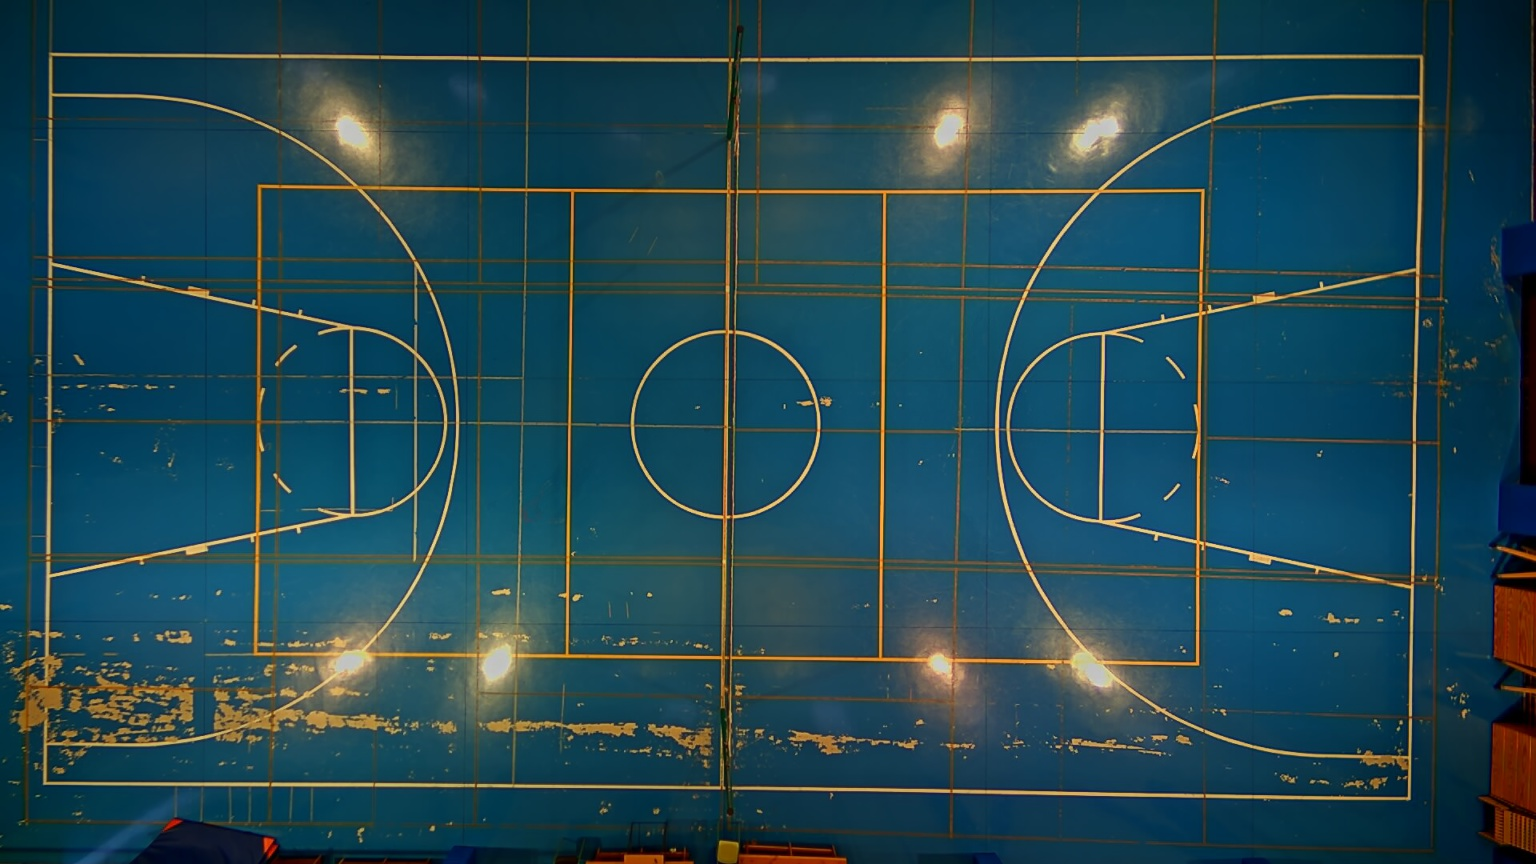
\includegraphics[width=0.6\textwidth]{images/campo}
    \caption{Imagen del campo vacío}
    \label{fig:campo}
\end{figure}

Una vez hecho esto, las posiciones de los jugadores y del balón deberían quedar registrados en un archivo CSV, divididas por jugadas y sets. Para hacer esta división, lo ideal es que funcione de forma automática, aunque lo podría hacer un operario mediante pulsaciones de teclas.

El proyecto parte suponiendo que la cámara mencionada ya ha sido instalada. Por tanto, los detalles de la instalación de la parte hardware y la extracción de imágenes del campo de juego quedan fuera del alcance del trabajo.


\subsection{Herramientas utilizadas y metodología}
Durante la realización de este trabajo se han utilizado una serie de herramientas que pasaré a listar y detallar a continuación.

\subsubsection*{Python}
Python es un lenguaje de programación interpretado, multiparadigma y de tipado dinámico. Nace a finales de los 80, pero alcanzó una mayor popularidad a partir de mediados de los 2000, poco después de la versión 2.0 del lenguaje. En la actualidad, Python es uno de los lenguajes más utilizados en materia de procesado científico y \textit{machine learning}.

La totalidad del desarrollo del software de este trabajo se realizará en este lenguaje. Se ha tomado esta decisión debido a la gran sencillez que aporta, en conjunto con el hecho de que es multiplataforma. Otra gran ventaja del lenguaje es la disponibilidad de librerías como OpenCV, que será la piedra angular del proyecto. 

\subsubsection*{OpenCV}
OpenCV surge en 1999, originalmente desarrollada por Intel, como librería de C++ de visión artificial y \textit{machine learning}. En la actualidad cuenta con versiones para Python, Java, MATLAB entre otros lenguajes. Se encuentra disponible para Linux, Mac y Windows. OpenCV cuenta con implementaciones de más de 2500 algoritmos de visión artificial, que cubren un gran abanico de casos de uso, desde reconocimiento de objetos hasta control de tráfico o seguridad.

Como se ha comentado antes, OpenCV es una parte fundamental de este proyecto, ya que todo lo referente a la visión artificial va a hacer uso de esta librería.

\subsubsection*{Git}
Git es una herramienta de control de versiones originalmente desarrollada por Linus Torvalds para mantener el kernel de Linux. Su desarrollo comienza en abril de 2005 y su primera versión estable se lanzó en diciembre de ese mismo año. En la actualidad se ha convertido en uno de los sistemas de control de versiones más importantes.

El uso de Git (o cualquier VCS) es, en mi opinión, indispensable por pequeña que sea la envergadura del proyecto a desarrollar, debido a la posibilidad de tener siempre disponibles las versiones anteriores del código. Esto hace extremadamente sencillo volver a una versión anterior en caso de necesidad, y proporciona una buena manera de hacer backups incrementales del código. También es muy útil de cara al trabajo en equipo, en nuestro caso, la supervisión de los avances del trabajo por parte del director.

\subsection*{PyQt}
PyQt es una adaptación multiplataforma de la librería gráfica Qt. Esta librería está desarrollada por la compañía inglesa Riverbank Computing. PyQt cuenta con toda la funcionalidad de programación de aplicaciones gráficas disponible en la librería de la que proviene.

PyQt ha facilitado en gran medida la programación de una interfaz gráfica, lo que es interesante de cara a facilitar el uso de la aplicación al usuario medio